%%%% SELECT ONE OF THE FOLLOWING COMMANDS %%%%%%%%

%%% TEMPLATE FOR PROCEEDINGS TRACK %%%%
\documentclass[mlmain,onecolumn]{jmlr}

%% TEMPLATE FOR Extended Abstract Track %%%%%%%
% \documentclass[mlabstract,onecolumn]{jmlr}

%%%%%%%%%%%%%%%%%%%%%%%%%%%%%%%%%%%%%%%%%%%%%%%%%

%%%%%%%%%%%%%%%%%%%%%%%%
% Watermark
%These 4 commands must be removed for the camera-ready version.
\usepackage[hpos=300px,vpos=70px]{draftwatermark}
\SetWatermarkText{\test}
\SetWatermarkScale{1}
\SetWatermarkAngle{0}
%%%%%%%%%%%%%%%%%%%%%%%%%%

% The following packages will be automatically loaded:
% amsmath, amssymb, natbib, graphicx, url, algorithm2e

\usepackage{booktabs}

%%%% DON'T CHANGE %%%%%%%%%
\jmlrvolume{}
\firstpageno{1}
\editors{List of editors' names}
\jmlryear{2026}
\jmlrworkshop{Symmetry and Geometry in Neural Representations}
%%%%%%%%%%%%%%%%%%%%%%%%%%%

% Notation macros
\newcommand{\X}{\mathcal{X}}
\newcommand{\A}{\mathcal{A}}
\newcommand{\R}{\mathbb{R}}
\newcommand{\E}{\mathbb{E}}
\newcommand{\conf}{c}
\newcommand{\dF}{\delta_{\!F}}
% Lean identifiers, typewriter, breakable after underscores
\newcommand{\leanid}[1]{{\def\_{\textunderscore\allowbreak}\texttt{#1}}}

\title[Truth Has a Boundary]{Truth Has a Boundary. A Machine-Verified
Topological Constraint on Models That Separate Truth from
Falsehood}

%%%%%%%%%%%%%%%%%%%%%%%%%%%%%%%%%%%%%
% THE MANUSCRIPT, DATA AND CODE MUST BE ANONYMIZED DURING THE REVIEW PROCESS.
% DON'T INCLUDE ANY INFORMATION ABOUT AUTHORS DURING THE REVIEW PROCESS.
%%%%%%%%%%%%%%%%%%%%%%%%%%%%%%%%%%%%%

\begin{document}

\maketitle

\begin{abstract}
Probing studies read truth off a language model's activations,
treating truth as a continuous decodable field over representation
space. We ask what the shape of that space requires of any model
answering over it. Our central result is a coupling theorem. If a
continuous model on a connected representation space ever answers
truly and ever answers falsely, and its confidence separates true
answers from false ones, then some query must carry confidence
exactly at the threshold while its answer sits exactly on the truth
boundary. The theorem mentions no safety guarantee, so it
does not depend on how a guarantee treats its own threshold. A
guarantee including its threshold is impossible, and one excluding
it survives but is silent at the coupled query. Under Lipschitz
regularity the coupled point sits inside an ambiguity tube of
computable width, any feasible system must carry strictly positive
truth-side slack, and for nonzero linear probes the truth boundary
is an affine hyperplane of codimension one. A symmetry version
needs no coverage assumption, a discrete analysis prices the
removal of topology, and multi-turn and stochastic extensions
follow, with the stochastic dichotomy deriving falsehood. We
machine-verify every theorem in Lean 4 against Mathlib with no
sorry placeholders, and the main results reduce to the three
standard kernel axioms. Experiments observe the predicted coupling
in five
small language models, with the model's own confidence signal and
against null baselines, and an adversarial attempt to train away
the slack plateaus strictly above zero.
\end{abstract}

\begin{keywords}
representational geometry, topology, uncertainty, calibration,
intermediate value theorem, Borsuk-Ulam, formal verification, Lean
\end{keywords}

\section{Introduction}
\label{sec:intro}

Truth is geometrically simple inside language models. Linear probes
separate true from false statements in activation space,
unsupervised methods find latent knowledge, and steering along
learned directions makes models more truthful
\citep{marks2024geometry,azaria2023internal,burns2023discovering,li2023inference,zou2023representation}.
All of this work treats truth as a continuous, decodable field over
representation space.

We take that picture seriously as geometry. Suppose truth is a
continuous scalar field on a connected representation space, and
the model's answers and confidences are continuous fields on the
same space, assumptions mentioning no architecture, training, or
scale, applying to any model whose fields are defined and
continuous on the stated domain. What they yield is a coupling
theorem. If the model ever answers
truly and ever answers falsely, and its confidence separates true
answers from false ones, then some query carries confidence exactly
at the threshold while its answer sits exactly on the truth
boundary (\figureref{fig:schematic}).

\begin{figure}[t]
\centering
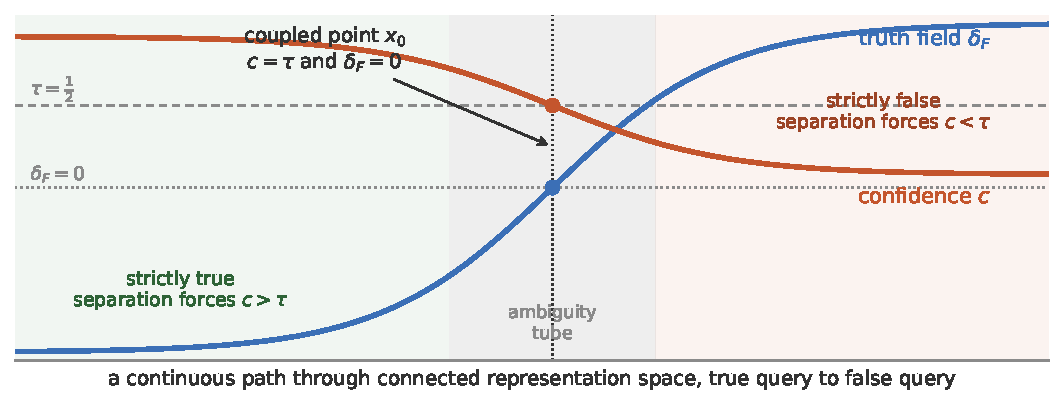
\includegraphics[width=0.64\linewidth]{schematic_coupling.pdf}
\caption{The coupling theorem in one picture. Along any true-to-false
path, separation forces confidence above $\tau$ on the strictly true
side and below on the strictly false side, so both fields must cross,
and the crossings coincide at the coupled point $x_0$ inside the
ambiguity tube of \theoremref{thm:width}.}
\label{fig:schematic}
\end{figure}

The proof is short, and the theorem's value lies in what it does
not mention, no safety guarantee and no threshold convention, so
every policy question becomes a corollary. An inclusive guarantee
is impossible, an exclusive one survives but says nothing at the
point topology guarantees, slack buys safety, and for the nonzero
linear probes used in practice the truth boundary is an affine
hyperplane.

\paragraph{Contributions.}
The boundary coupling theorem with its corollary taxonomy
(\sectionref{sec:coupling}); the geometry of the boundary, closed,
crossed by every true-to-false path, a hyperplane for nonzero
linear probes, with an ambiguity tube of strictly positive
truth-side slack (\sectionref{sec:geometry}); a symmetry version
needing no coverage (\sectionref{sec:antipodal}); a discrete
analysis with multi-turn and stochastic extensions
(\sectionref{sec:discrete}); and full machine verification
(\sectionref{sec:lean}, \tableref{tab:lean}).

The mathematics is elementary, and the contribution is not
technical difficulty. It is a framing in which exact threshold
uncertainty is a topological property of representation space,
precision, since the theorems name every assumption in play, and
verification, since we machine-check every statement, leaving the
premises as the only thing to argue about. The theorems do not say
models err often, and the coupled point is neither strictly true
nor strictly false.

\paragraph{Related work.}
Statistical and computability arguments make hallucination
inevitable in other senses
\citep{kalai2024calibrated,kalai2025why,xu2024hallucination}; ours
is topological and yields uncertainty rather than confident
falsehood. The probing literature models truth as a continuous
decodable field
\citep{marks2024geometry,burns2023discovering,azaria2023internal,li2023inference,zou2023representation,park2024linear},
exactly our hypothesis on $\delta$, and our results give that
program a frontier. Connected-domain modeling follows the manifold
hypothesis \citep{fefferman2016testing,cai2021isotropy}, and the
symmetry section is a scalar relative of Borsuk-Ulam
\citep{borsuk1933drei,matousek2003using}. To our knowledge this is
the first fully machine-verified impossibility-style result on
model truthfulness at the level of representation geometry
\citep{moura2021lean,mathlib2020}. \appendixref{app:extended}
extends all four threads.

\section{The setting}
\label{sec:setting}

$\X$ is a topological space of queries as the model represents
them, prompt embeddings or residual-stream states, $\A$ a
topological space of answers, and our standing assumption is simple.

\begin{quote}
\textbf{(T)} $\X$ is connected and nonempty.
\end{quote}

Standard practice models ambient embedding spaces as $\R^d$ or
connected submanifolds, satisfying (T), though a token-driven
model's reachable set may be disconnected. When guarantees range
over the ambient space, as they do whenever a probe or steering
vector applies at arbitrary points, (T) holds. Continuity likewise
idealizes trained networks, softmax and embeddings being continuous
while argmax decoding is not, and \sectionref{sec:discrete} prices
dropping either idealization.

\begin{definition}[Model and truth fields]
\label{def:model}
A \emph{model} is a map $F = (a, \conf)$ from $\X$ to
$\A \times \R$, with answer $a(x)$ and scalar confidence $\conf(x)$,
\emph{continuous} if both components are. A \emph{truth field} is a
continuous $\delta$ from $\X \times \A$ to $\R$, a signed
truth-distance, negative on strictly true answers, positive on
strictly false ones, with the \emph{truth boundary} as its zero set.
The \emph{realized truth field} is $\dF(x) = \delta(x, a(x))$.
\end{definition}

A linear probe $w^\top x - b$ on activations
\citep{marks2024geometry,burns2023discovering} is a candidate
continuous $\dF$, its zero set the probe's classification boundary.
Whether that coincides with semantic truth away from the fitted
samples is an empirical premise, not a theorem, and our results
hold under it.

\begin{definition}[Truth-separating at threshold $\tau$]
\label{def:separating}
Fix a threshold $\tau$, a truth slack $\varepsilon \ge 0$, and a
confidence margin $\gamma \ge 0$. $F$ is
\emph{$(\varepsilon, \gamma)$-separating at $\tau$} if
$\dF(x) < -\varepsilon$ implies $\conf(x) > \tau + \gamma$ and
$\dF(x) > \varepsilon$ implies $\conf(x) < \tau - \gamma$. The slack
is in units of $\dF$ and the margin in units of $\conf$, so the
condition survives independent rescaling. \emph{Exactly separating}
means both are zero.
\end{definition}

\begin{definition}[Covering]
\label{def:covering}
$F$ is \emph{$\varepsilon$-covering} if some query has
$\dF < -\varepsilon$ and some has $\dF > \varepsilon$, at
$\varepsilon = 0$ somewhere strictly right and somewhere strictly
wrong.
\end{definition}

\begin{definition}[Guarantees]
\label{def:guarantees}
A \emph{threshold-inclusive guarantee} says that
$\conf(x) \ge \tau$ implies $\dF(x) < 0$, and a
\emph{threshold-exclusive} one that $\conf(x) > \tau$ implies
$\dF(x) < 0$.
\end{definition}

Any model ever right and ever wrong satisfies covering,
separation idealizes a perfect truth probe used as confidence, the
guarantees idealize mitigation, the coupling results hold at any
threshold, and the biconditional variants sit at one half.

\begin{remark}[This is not statistical calibration]
\label{rem:calibration}\sloppy
Separation is pointwise and much stronger than statistical
calibration \citep{guo2017calibration}, and one-way by construction.
The \emph{biconditional} variant adds the converses, so the sign of
$\dF$ and the side of the threshold determine each other. The
symmetry and discrete results use it, and it implies the one-way
pair, Lean
\leanid{strictCalibrated\_to\_epsCalibrated\_zero\_half}.
\end{remark}

\section{The boundary coupling theorem}
\label{sec:coupling}

Topology enters through one theorem needing no confidence.

\begin{theorem}[Boundary existence]
\label{thm:boundary}
Let $\X$ satisfy (T), the answer map and truth field be continuous,
and $F$ be $0$-covering. Then some $x_0$ has $\dF(x_0) = 0$, since
$\dF$ is continuous with both signs and the IVT applies on the
connected space. Lean \leanid{model\_truth\_boundary\_nonempty}, IVT
step \leanid{IsPreconnected.intermediate\_value2}.
\end{theorem}

\begin{theorem}[Boundary coupling]
\label{thm:coupling}
Let $\X$ satisfy (T). Let $\conf$ be continuous, and let $F$ be
$0$-covering and exactly separating at $\tau$. Then some $x_0$
satisfies both
\[
\conf(x_0) = \tau \qquad\text{and}\qquad \dF(x_0) = 0 .
\]
\end{theorem}

\begin{proof}
Separation converts the coverage witnesses into confidence
witnesses on both sides of $\tau$, and the IVT gives $x_0$ with
$\conf(x_0) = \tau$. Were $\dF(x_0)$ negative, separation would give
$\conf(x_0) > \tau$, and positive, $\conf(x_0) < \tau$, so
$\dF(x_0) = 0$. This is Lean theorem \leanid{boundary\_coupling}.
\end{proof}

The theorem mentions no guarantee, so no threshold convention
affects it. We call such an $x_0$ a \emph{coupled point}
(\figureref{fig:schematic}), and what it means for safety is
policy, with each policy a corollary.

\begin{corollary}[Policy taxonomy]
\label{cor:policy}
Adding a threshold-inclusive guarantee to
\theoremref{thm:coupling}'s hypotheses is jointly contradictory,
the trilemma, since coverage, exact separation, and an inclusive
guarantee cannot jointly hold. Adding a threshold-exclusive
guarantee yields no contradiction, but the coupled point satisfies
$\conf(x_0) = \tau$, its antecedent fails exactly there, and the
system owns a boundary query about which its guarantee says
nothing. Lean theorems \leanid{closed\_guarantee\_impossible},
\leanid{hallucination\_trilemma}, and
\leanid{open\_guarantee\_silent}.
\end{corollary}

Defining the guarantee with a strict inequality therefore does not
dissolve the impossibility. The coupling theorem is convention-free,
the convention only selects which clause of the taxonomy applies,
and the coupled point exists under either convention.

\section{The geometry of the boundary}
\label{sec:geometry}

\begin{theorem}[Closed, and crossed by every path]
\label{thm:closed}
For any topological $\X$ and $\A$, continuous $\delta$ and answer
map, $\{x \mid \dF(x) = 0\}$ is closed in $\X$, and any continuous
path from a query answered strictly truly to one answered strictly
falsely contains a point exactly on the truth boundary. Lean
theorems \leanid{model\_truth\_boundary\_isClosed} and
\leanid{path\_crosses\_truth\_boundary}.
\end{theorem}

\begin{theorem}[Linear probes have hyperplane boundaries]
\label{thm:hyperplane}
Let $f$ be a nonzero linear probe on a $d$-dimensional real space
with offset $b$. Then $\{x \mid f(x) = b\}$ is an affine translate
of the kernel of $f$, of dimension exactly $d - 1$. Lean theorems
\leanid{linear\_probe\_boundary\_coset} and
\leanid{linear\_probe\_boundary\_dim}, by rank-nullity.
\end{theorem}

\begin{theorem}[Nonlinear boundaries are hyperplanes to first order]
\label{thm:nonlinear}
Let $f$ be differentiable at a boundary point $x_0$ of a
$d$-dimensional real space, with nonzero derivative $L$. Then every neighborhood of $x_0$ contains strictly
true and strictly false points, and for every $\varepsilon > 0$
some $\delta > 0$ has every boundary point $x$ within $\delta$
satisfying $|L(x - x_0)| \le \varepsilon \|x - x_0\|$, deviating
sublinearly from the tangent hyperplane $x_0 + \ker L$ of dimension
$d - 1$. Lean theorems \leanid{regular\_point\_is\_crossing},
\leanid{nonlinear\_boundary\_tangent}, and
\leanid{tangent\_hyperplane\_dim}.
\end{theorem}

The hyperplane picture therefore survives nonlinearity to first
order, every regular point a sign crossing generating local coverage
for free against a codimension-one tangent hyperplane. Next we
quantify what slack changes.

\begin{theorem}[Corridor and tube]
\label{thm:width}
Let $\conf$ be $L_c$-Lipschitz and $\dF$ be $L_\delta$-Lipschitz.
For $\gamma > 0$, queries with $\conf \ge \tau + \gamma$ and with
$\conf \le \tau - \gamma$ are at distance at least $2\gamma/L_c$,
and for a coupled point $x_0$, every query within distance $r$ of
$x_0$ has truth margin at most $L_\delta \, r$ and confidence
within $L_c \, r$ of the threshold. Lean theorems
\leanid{confidence\_gap\_width}, \leanid{ambiguity\_tube}, and
\leanid{truth\_margin\_tube}.
\end{theorem}

The coupled point therefore centers a tube of near-ambiguous
queries, decisive regions no closer than the corridor width.

\begin{theorem}[Approximate coupling, and slack must be positive]
\label{thm:approx}
Let $\X$ satisfy (T), let $\conf$ be continuous, and let $F$ be
$\varepsilon$-covering, $(\varepsilon, \gamma)$-separating at
$\tau$, and carry a threshold-inclusive guarantee. Then some $x_0$
has $\conf(x_0) = \tau$ and $-\varepsilon \le \dF(x_0) < 0$, and
consequently the truth slack satisfies $\varepsilon > 0$ for every
margin $\gamma \ge 0$, so zero truth slack is infeasible. These are
Lean theorems \leanid{two\_slack\_approx\_coupling},
\leanid{exact\_from\_approx}, and
\leanid{truth\_slack\_must\_be\_positive}.
\end{theorem}

Slack is therefore a geometric budget, positivity attaching to the
truth side alone. We read the infimum of feasible truth slack as
the system's truth-boundary width, with the relative width of
\sectionref{sec:experiments} as a dimensionless proxy, and under
the guarantee no query with confidence between $\tau$ and
$\tau + \gamma$ sits exactly on the boundary (Lean
\leanid{no\_boundary\_in\_upper\_band\_two\_slack}).

\section{Symmetry replaces coverage}
\label{sec:antipodal}

Symmetry can replace coverage. Suppose semantic negation acts on
$\X$ as a continuous involution $\sigma$ with no fixed point and
the realized truth field is odd under it, idealizing negation's
measured reflection of truth directions \citep{marks2024geometry}.

\begin{theorem}[Odd fields vanish]
\label{thm:odd-zero}
Let $\X$ satisfy (T) with such an action $\sigma$, and let $g$ be
continuous and odd under $\sigma$. Then $g$ has a zero, by the IVT
between any $x$ and $\sigma x$. This is Lean theorem
\leanid{antipodal\_odd\_has\_zero}.
\end{theorem}

This is the scalar shadow of Borsuk-Ulam, needing no sphere. Two
refinements make it robust and concrete.

\begin{theorem}[Robust and concrete oddness]
\label{thm:approx-odd}
Let $\X$ satisfy (T), $\sigma$ map $\X$ to itself, and $g$ be
continuous with $|g(\sigma x) + g(x)| \le \varepsilon$ for all $x$.
Then some $x$ has $|g(x)| \le \varepsilon/2$. Moreover, on the unit
sphere of $\R^d$, $d \ge 2$, with negation the antipodal map, every
continuous odd field vanishes somewhere on the sphere. Lean theorems
\leanid{approx\_odd\_near\_zero} and \leanid{sphere\_odd\_has\_zero}.
\end{theorem}

The near-boundary point degrades linearly with the defect, and the
sphere is, up to a learned affine map, where layer normalization
places its states, negation the candidate antipode.

\begin{theorem}[Antipodal coupling]
\label{thm:antipodal}
Let $\X$ satisfy (T) with a free continuous involution $\sigma$,
$F$ be continuous with biconditional separation at $\tfrac12$, and
$\dF$ be odd. Then some $x$ has $\conf(x) = \tfrac12$ and
$\dF(x) = 0$. Lean \leanid{antipodal\_hallucination\_trilemma}.
\end{theorem}

No coverage hypothesis appears, so a negation-closed family of
questions meets the truth boundary by symmetry alone. Equivariance,
usually a design virtue \citep{bronstein2021geometric}, is here the
engine of the obstruction.

\section{Leaving the continuum, adding turns and randomness}
\label{sec:discrete}
\label{sec:extensions}

Token spaces are finite, and one may object that connectedness does
illegitimate work. The discrete analysis prices the objection, since
without topology we must assume the boundary witness rather than
derive it.

\begin{theorem}[Discrete impossibility]
\label{thm:discrete}
Let $\X$ and $\A$ be arbitrary sets with arbitrary $F$ and
$\delta$, with biconditional separation at $\tfrac12$. If some query
has $\dF = 0$, a threshold-inclusive guarantee fails, and such a
guarantee is possible exactly when no boundary query exists. These
are Lean theorems
\leanid{boundary\_question\_impossible} and
\leanid{faithful\_iff\_boundary\_free}.
\end{theorem}

The assumed witness is what connectedness derived free in
\theoremref{thm:boundary}, and without it a crossing survives.

\begin{proposition}[Discrete sign change]
\label{prop:discrete-ivt}
Let $g$ map $\{0, \dots, n\}$ to $\R$ with $g(0) < 0 < g(n)$. Then
some $i$ has $g(i) < 0 \le g(i+1)$. This is Lean theorem
\leanid{discrete\_sign\_change}.
\end{proposition}

Along any token path from true to false, $\dF$ crosses zero between
adjacent steps, a straddling pair rather than a boundary state,
hence no contradiction alone. The continuum upgrades the
crossing into a witness. Interaction does not escape, since $\X^T$
is connected and the arguments transport verbatim
(\leanid{multi\_turn\_history\_dependent}). Nor does randomization.
On the expected fields the coupling theorem yields expected
confidence one half at expected truth-distance zero
(\leanid{stochastic\_coupling\_expected}), and a dichotomy converts
expectation into sampling behavior.

\begin{theorem}[Stochastic dichotomy]
\label{thm:dichotomy}
Let $(\Omega, \mu)$ be a probability space and let $c, d$ be real
functions on $\Omega$ with $d$ integrable and of mean zero. Suppose
sample faithfulness holds almost everywhere, meaning
$c \ge \tfrac12$ implies $d < 0$, and suppose
$\mu\{c \ge \tfrac12\} > 0$. Then $\mu\{d > 0\} > 0$. This is Lean
theorem \leanid{stochastic\_dichotomy}.
\end{theorem}

A model faithful on almost every sample and confident with positive
probability at a coupled point must emit strictly false answers with
positive probability. Randomization spreads the boundary across
samples, and here alone the theory derives falsehood.

\paragraph{Machine verification.}
\phantomsection\label{sec:lean}
Every theorem and proposition corresponds to a named, sorry-free
Lean 4 result \citep{moura2021lean,mathlib2020}. The artifact
builds with zero errors, axiom audits reduce each main theorem to
the three standard kernel axioms, \tableref{tab:lean} maps every
result to its identifier, and the prose claims nothing beyond the
formal statements.

\section{Empirical illustration}
\label{sec:experiments}
\phantomsection\label{app:experiment}

We checked whether the idealized theory is visible in five open
models, GPT-2 (124M), Pythia-410M, Qwen2.5-0.5B, Phi-1.5 (1.3B),
and Qwen2.5-1.5B, on the 1496 matched city statements and negations
of \citet{marks2024geometry}. We embed each statement at its final
token, select the layer whose probe validates best, train the truth
field $\dF$ as a linear logistic probe on one city split and the
confidence field $\conf$ as a second head on a disjoint split with
a different seed, independently trained readouts of the same space,
the canonical construction the theory models. We interpolate hidden
states from each true statement to its negation, record both
fields, and keep paths whose endpoints the probe classifies
correctly, 83, 104, 137, 66, and 148 paths, holding test cities out
of both splits.

\begin{table}[t]
\centering
\caption{Boundary coupling and null calibration in five small
models. Probe and Head are held-out accuracies, Verbal the model's
own answer accuracy, Cross the mean confidence at the probe's zero
crossing, Gap the median crossing distance as a fraction of the
path, Width the relative boundary width, Decisive the
endpoint-decisive paths of the endogenous field, Endo its median
gap on them, Perm and Rand the median null gaps over twenty seeds.}
\label{tab:experiment}
\label{tab:endogenous}
\footnotesize
\setlength{\tabcolsep}{4pt}
\begin{tabular}{lccccccccccc}
\toprule
Model & Layer & Probe & Head & Verbal & Cross & Gap & Width &
Decisive & Endo & Perm & Rand \\
\midrule
GPT-2 (124M) & 9/12 & 0.77 & 0.72 & 0.48 & 0.52 & 0.25 & 0.33 &
23/53 & 0.23 & 0.48 & 0.33 \\
Pythia-410M & 18/24 & 0.82 & 0.77 & 0.50 & 0.51 & 0.20 & 0.36 &
0/84 & none & 0.45 & 0.45 \\
Qwen2.5-0.5B & 12/24 & 0.96 & 0.96 & 0.71 & 0.49 & 0.10 & 0.20 &
128/137 & 0.13 & 0.43 & 0.40 \\
Phi-1.5 (1.3B) & 18/24 & 0.72 & 0.72 & 0.56 & 0.43 & 0.31 & 0.37 &
53/80 & 0.40 & 0.48 & 0.38 \\
Qwen2.5-1.5B & 14/28 & 1.00 & 1.00 & 0.96 & 0.54 & 0.05 & 0.11 &
146/147 & 0.08 & 0.45 & 0.45 \\
\bottomrule
\end{tabular}
\end{table}

\begin{figure}[t]
\centering
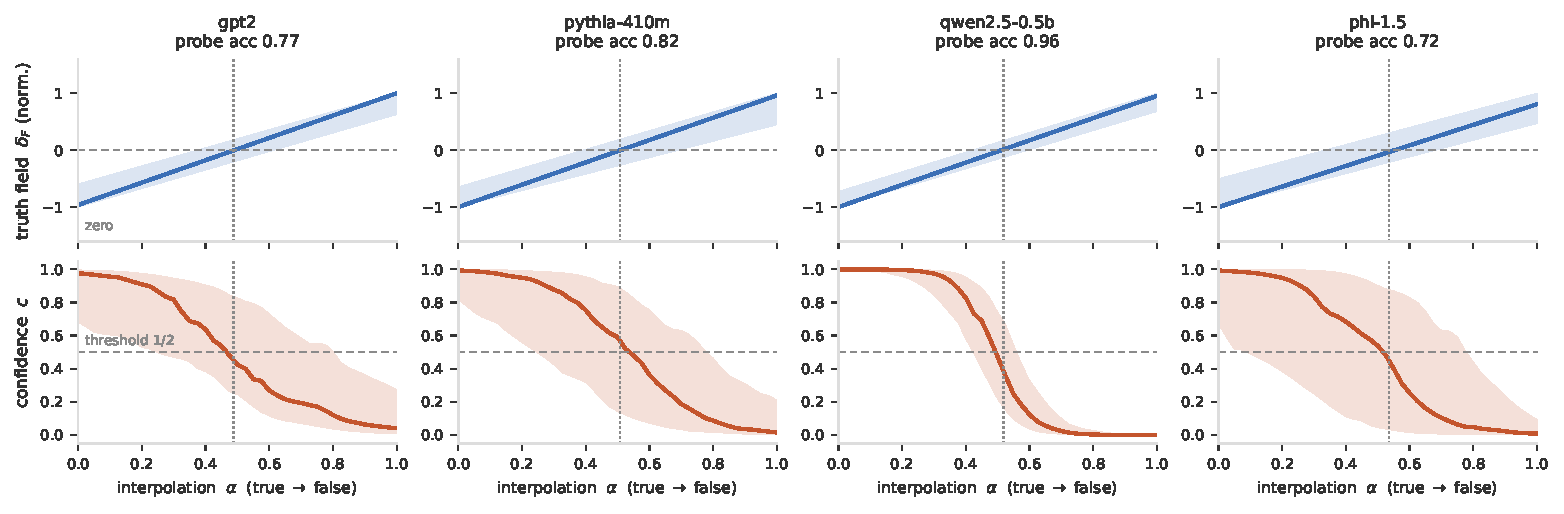
\includegraphics[width=0.54\linewidth]{boundary_coupling.pdf}\\[2pt]
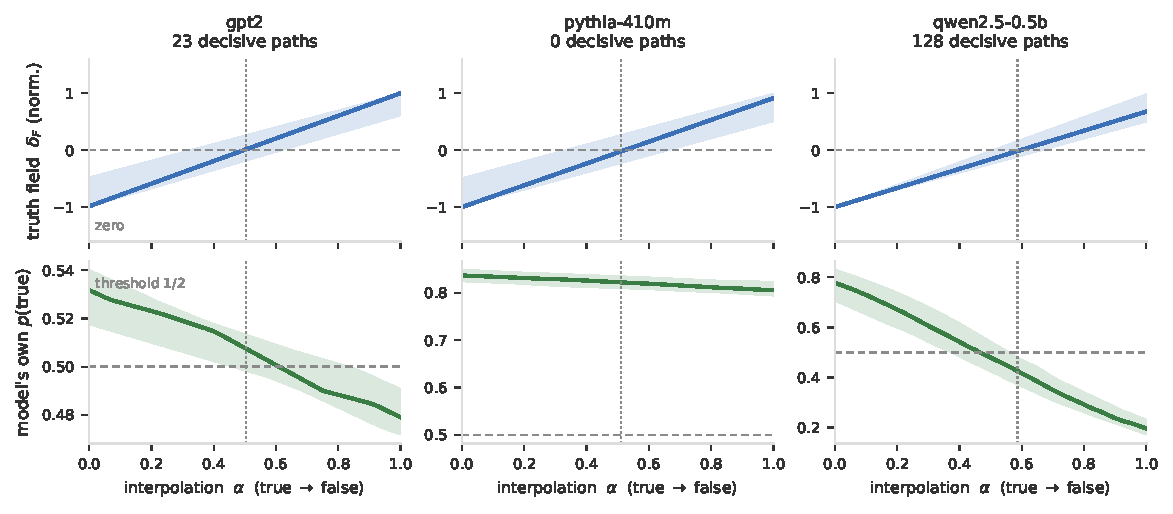
\includegraphics[width=0.54\linewidth]{endogenous_coupling.pdf}
\caption{Upper pair of rows, the truth probe (normalized, median and
interquartile band) and the independently trained confidence along
true-to-negation paths, the dotted line marking the mean probe zero
crossing where confidence passes near one half. Lower pair,
the same with the model's own probability of answering true from
patched final-block states, decisive paths where any exist. The
Qwens sweep through one half at the boundary, Pythia-410M answers
true everywhere so the premise fails, and GPT-2 and Phi-1.5 sit
between.}
\label{fig:coupling}
\end{figure}

\paragraph{Findings.}
\tableref{tab:experiment} and \figureref{fig:coupling} summarize.
Probes separate truth at 0.72 to 1.00 while only the Qwens
verbalize it above chance, 0.71 and 0.96 against 0.48 to 0.56, the
known represented-verbalized gap. Every kept path shows the
predicted adjacent sign change, mean confidence at the probe's zero
crossing is 0.52, 0.51, 0.49, 0.43, and 0.54, and the gap between
the two crossings tracks probe accuracy monotonically, from 0.31 for
Phi-1.5, the weakest probe, to 0.05 for Qwen2.5-1.5B, the
strongest. The ordering follows separation, not parameter count,
since Phi-1.5 outweighs all but Qwen2.5-1.5B yet separates worst,
a sweep of all its 24 layers topping out at 0.73 test accuracy,
while the Qwen pair
shows scale helping through separation, probe 0.96 to 1.00 and the
gap halved. The relative boundary width, median $|\dF|$ where
confidence is in $[0.4, 0.6]$ over endpoint scale, runs 0.37 to
0.11, and the kNN graph keeps true and false in one shared main
component in all five models, though three show a second component,
identified below.

\paragraph{The model's own confidence.}
Both fields above target truth, so we repeat the experiment with a
confidence field the model supplies itself, no trained head, read
through unembedding weights fixed by pretraining. We capture the
final block's last-token state under a question template,
interpolate as before, patch the state back in, and read the
model's own probability of answering true, the probe trained on a
disjoint split of the same states, 53, 84, 137, 80, and 147 kept
paths. A path satisfies the separation premise when this field sits
on the correct side of one half at both endpoints. \tableref{tab:endogenous} and \figureref{fig:coupling} report
the result. Qwen2.5-1.5B meets the premise on 146 of 147 paths at
gap 0.08 and Qwen2.5-0.5B on 128 of 137 at 0.13, against nulls of
0.40 and above. Pythia-410M answers true regardless, so the premise
fails everywhere and the theory predicts nothing. GPT-2 (23 of 53
decisive) and Phi-1.5 (53 of 80, verbal 0.56) have gaps at null, so
endpoint decisiveness without verbal capability is not separation.
Coupling with the model's own uncertainty appears cleanly where the
premise holds throughout, and never where it fails.


\paragraph{Null baselines.}
Permuted-label and random-direction heads, twenty seeds each on
the same kept paths, calibrate the gaps
(\tableref{tab:endogenous}). The trained-head gaps of 0.25, 0.20,
0.10, 0.31, and 0.05 fall below every null median, and below the
entire null range for Pythia-410M and both Qwens, while GPT-2 and
Phi-1.5 sit inside the random-head range, weak evidence alone.
Bootstrap 95 percent intervals over ten thousand path resamples are
0.175 to 0.325, 0.15 to 0.287, 0.10 to 0.125, 0.175 to 0.375, and
0.05 to 0.075, with 0.10 to 0.15 and 0.075 to 0.10 for the Qwens'
endogenous fields, every upper bound at or below its null median except
endogenous GPT-2 and Phi-1.5.

\paragraph{A second dataset.}
The same pipeline on the 354 Spanish-English translation pairs from
the same source replicates in both Qwens, probes 0.98 and 0.94 with
gaps 0.05 and 0.10, while Pythia-410M and Phi-1.5 drop to probes
0.70 and 0.71 with gaps at null and GPT-2 is at chance with too few
paths to score, so coupling again appears exactly where separation
holds.

\paragraph{What the second component is.}
Where a second kNN component appears it splits exactly by surface
form, positives in one and negations in the other, with true and
false in equal measure inside each. Syntax separates activations,
not truth, and the interpolation paths are ambient line segments,
connected regardless of clustering.

\paragraph{Measuring the oddness defect.}
The matched pairs also measure the oddness premise of
\sectionref{sec:antipodal}. The defect $|\dF(x) + \dF(\sigma x)|$
relative to endpoint scale has median 0.40, 0.43, 0.30, 0.53, and
0.17, smallest for the strongest model. Exact oddness fails, which
is why \theoremref{thm:approx-odd} carries the approximate
version, whose near-boundary point survives any defect. The width
column of \tableref{tab:experiment} likewise gives the slack
diagnostic of \sectionref{sec:geometry} an empirical proxy, 0.11
to 0.37.

\paragraph{Nonlinear probes.}
A linear truth field crosses zero along a linear path by
construction, so we replace both fields with one-hidden-layer MLPs
on the same splits, removing that guarantee and the hyperplane
boundary. The MLP probes reach 0.79, 0.87, 0.97, 0.80, and 1.00
with 124, 121, 144, 104, and 149 kept paths, every path still
crosses zero, and at least 98 percent cross exactly once, each
crossing the clean sign change \theoremref{thm:nonlinear} derives
at regular points. The coupling tightens or holds, gaps 0.15, 0.20,
0.075, 0.175, and 0.05, confidence at the crossing 0.42, 0.50,
0.42, 0.38, and 0.49, so the coupling is not an artifact of
linearity.

\paragraph{An adversarial falsification attempt.}
The strongest test of an impossibility result is a maximally
empowered attempt to violate it. We freeze the truth field, train a
confidence head on the forbidden objective, above one half where
the field says true and below elsewhere, guarantee weighted five to
one, on all non-test statements plus fresh interpolants each epoch,
and evaluate on 21{,}000 to 30{,}000 held-out path points per
model. \theoremref{thm:approx} predicts a positive slack floor,
boundary-localized failures, and a trade against guarantee
violations, and all three appear. The slack plateaus between 0.22
and 0.91 of endpoint scale, exactly flat over Qwen2.5-0.5B's final
fifteen epochs, never zero; median failing depth shrinks from 0.40
or more to 0.04 to 0.11, concentrating in the boundary tube; and
guarantee violations persist. The theorem forbids only exactly zero
slack for a fixed head, \theoremref{thm:width} pricing the escape,
so the plateau reflects this adversary's regularity and sharpening
only thins the tube around a boundary that does not go away.

\paragraph{What this does and does not show.}
The premises hold to varying degrees, disjoint splits rule out
shared training data, the nonlinear replication removes the
analytic sign-change guarantee, and the endogenous experiment
addresses the shared-target concern where the model verbalizes
truth. Code, data, and results are in the supplementary material.





\section{Discussion}
\label{sec:discussion}

The theorem rests on connectedness, continuity, coverage, and
separation, the trilemma adding an inclusive guarantee, and each
hypothesis admits relaxation at a named price
(\appendixref{app:extended}). Refusal training is connectedness
surgery, restricting to reachable queries is the same move while
probing and steering deploy over the ambient space, and dropping
continuity keeps only the adjacent crossing. The recommended stance
is band separation (\theoremref{thm:approx}), the infimum of
feasible truth slack a measurable diagnostic. The results are
existence statements, so nothing follows about error rates,
\theoremref{thm:dichotomy} alone derives falsehood, and the truth
field idealizes probe behavior, \theoremref{thm:approx-odd} pricing
oddness. With \theoremref{thm:nonlinear} and the scalar
Borsuk-Ulam analog verified, what remains is the full theorem for
jointly odd axes \citep{engels2025not}.

% Acknowledgments omitted for anonymous review.

\bibliography{neurreps_truth_boundary}

\appendix

\section{Extended discussion and related work}
\label{app:extended}

\paragraph{Hallucination inevitability.}
\citet{kalai2024calibrated} show statistically that calibrated
models must hallucinate on facts seen once in training,
\citet{kalai2025why} extend this line, and
\citet{xu2024hallucination} give a computability-theoretic
inevitability argument. Our mechanism is topological, lives in
representation space, localizes the conclusion at the truth
boundary, and is more modest, since the deterministic theorems
yield uncertainty rather than confident falsehood.

\paragraph{Geometry of truth in representations.}
Linearly decodable truth \citep{marks2024geometry}, unsupervised
latent-knowledge discovery \citep{burns2023discovering}, lie
detection from internal states \citep{azaria2023internal}, and
causal steering along truth directions
\citep{li2023inference,zou2023representation} all model truth as a
continuous decodable field on activation space, and the linear
representation hypothesis formalizes concepts as directions in that
space \citep{park2024linear}, and the literature treats confidence
signals \citep{farquhar2024detecting,kadavath2022language} the same
way. Topological analyses of networks
\citep{naitzat2020topology,hensel2021survey} and geometric deep
learning \citep{bronstein2021geometric} engineer or analyze such
structure, and we derive constraints from it.

\paragraph{Disconnect the space.}
Abstention breaks the argument at the IVT step, since declining to
answer on an open region deletes it from the domain and can
disconnect the true region from the false region. Refusal training,
on this reading, is connectedness surgery. Under the symmetry
version the cut must separate every representation from its
negation image, so piecemeal refusal is not enough.

\paragraph{Quantify only over reachable queries.}
The coupled point may be an ambient activation that no real prompt
produces, and a guarantee quantified only over reachable
representations is then untouched. The objection is fair, and it is
the domain version of disconnecting the space. But probing and
steering pipelines apply their readouts at interpolated and edited
activations, which is deployment over the ambient space, and a
guarantee over the uncertified reachable set inherits every unknown
of that set. Restricting the domain is a coherent stance if stated
as one.

\paragraph{Give up coverage or continuity.}
A model that never answers strictly falsely escapes. That is
vacuous for general-purpose systems and meaningful for
retrieval-grounded ones restricted to verified content. Dropping
continuity also escapes, at the price computed in
\sectionref{sec:discrete}, where only the adjacent-crossing
statement survives unconditionally.

\paragraph{Implications for probing and steering.}
Truth-probe pipelines posit a continuous $\dF$, and steering moves
representations relative to its zero set
\citep{li2023inference,zou2023representation}. Completing such a
pipeline over a connected domain with both truth values realized
yields an exact-uncertainty point on the probe's own boundary, a
hyperplane for linear probes, and mitigation effort should go
there.

\section{Formal statement conventions}
\label{app:conventions}

The Lean formalization states results over arbitrary topological
spaces \texttt{Q} and \texttt{A}, with a \texttt{ConnectedSpace}
instance on \texttt{Q}, a model \texttt{M} from \texttt{Q} to
\texttt{A x R}, and a truth field \texttt{delta} on \texttt{Q x A}
(rendered here in ASCII). The realized truth field is
\begin{center}
\texttt{fun q => delta (q, (M q).1)}
\end{center}
and confidence is \texttt{(M q).2}. We name the main conditions as
follows, and some identifiers retain historical names.

\begin{itemize}
\item \leanid{TwoSlackSeparating M delta c eps gamma} is separation
  at threshold \texttt{c} with truth slack \texttt{eps} and
  confidence margin \texttt{gamma}. The equal-slack case is
  \leanid{EpsCalibrated M delta c eps}, definitionally
  (\leanid{epsCalibrated\_iff\_twoSlack}).
\item Covering with slack \texttt{eps} is
  \leanid{EpsCovering M delta eps}.
\item The biconditional variant at threshold one half is
  \leanid{StrictCalibrated M delta}.
\item The threshold-inclusive guarantee at threshold one half is
  \leanid{TrilemmaFaithful M delta}. The general threshold version
  appears inline in the theorems that use it.
\end{itemize}

The embedding-space instantiation uses
\texttt{EuclideanSpace R (Fin d)}. The quantitative results use
\texttt{PseudoMetricSpace} and explicit Lipschitz hypotheses, and the
hyperplane results use \texttt{LinearMap} with rank-nullity.

\begin{table}[htbp]
\centering
\caption{Every result in the paper and its machine-checked counterpart.}
\label{tab:lean}
\footnotesize
\begin{tabular}{l@{\hspace{1em}}p{8.2cm}}
\toprule
Result & Lean identifier \\
\midrule
Thm.~\ref{thm:boundary} & \leanid{model\_truth\_boundary\_nonempty} \\
Thm.~\ref{thm:coupling} & \leanid{boundary\_coupling} \\
Cor.~\ref{cor:policy} & \leanid{closed\_guarantee\_impossible},
  \leanid{hallucination\_trilemma},
  \leanid{open\_guarantee\_silent} \\
Thm.~\ref{thm:closed} & \leanid{model\_truth\_boundary\_isClosed},
  \leanid{path\_crosses\_truth\_boundary} \\
Thm.~\ref{thm:hyperplane} & \leanid{linear\_probe\_boundary\_coset},
  \leanid{linear\_probe\_boundary\_dim} \\
Thm.~\ref{thm:nonlinear} & \leanid{regular\_point\_is\_crossing},
  \leanid{nonlinear\_boundary\_tangent},
  \leanid{tangent\_hyperplane\_dim} \\
Thm.~\ref{thm:width} & \leanid{confidence\_gap\_width},
  \leanid{ambiguity\_tube}, \leanid{truth\_margin\_tube} \\
Thm.~\ref{thm:approx} & \leanid{two\_slack\_approx\_coupling},
  \leanid{exact\_from\_approx},
  \leanid{truth\_slack\_must\_be\_positive} \\
Upper-band exclusion & \leanid{no\_boundary\_in\_upper\_band\_two\_slack} \\
Thm.~\ref{thm:odd-zero} & \leanid{antipodal\_odd\_has\_zero} \\
Thm.~\ref{thm:approx-odd} & \leanid{approx\_odd\_near\_zero},
  \leanid{sphere\_odd\_has\_zero} \\
Thm.~\ref{thm:antipodal} & \leanid{antipodal\_hallucination\_trilemma} \\
Thm.~\ref{thm:discrete} & \leanid{boundary\_question\_impossible},
  \leanid{faithful\_iff\_boundary\_free} \\
Prop.~\ref{prop:discrete-ivt} & \leanid{discrete\_sign\_change} \\
Multi-turn & \leanid{multi\_turn\_history\_dependent} \\
Stochastic expected-value coupling & \leanid{stochastic\_coupling\_expected} \\
Thm.~\ref{thm:dichotomy} & \leanid{stochastic\_dichotomy} \\
Bundled master theorem & \leanid{hallucination\_master\_theorem} \\
Definitional bridges &
  \leanid{strictCalibrated\_to\_epsCalibrated\_zero\_half},
  \leanid{epsCalibrated\_iff\_twoSlack} \\
\bottomrule
\end{tabular}
\end{table}

\section{Core proof term}
\label{app:leanproof}

The Lean proof of the coupling theorem, lightly annotated and
rendered in
ASCII.

\begin{verbatim}
theorem boundary_coupling
    {Q A : Type*} [TopologicalSpace Q] [ConnectedSpace Q]
    [TopologicalSpace A]
    (M : Q -> A x R) (delta : Q x A -> R) (c : R)
    (hconf : Continuous (fun q => (M q).2))
    (hcov : EpsCovering M delta 0)
    (hcal : EpsCalibrated M delta c 0) :
    exists q0, (M q0).2 = c /\ delta (q0, (M q0).1) = 0 := by
  obtain <<qt, ht>, <qf, hf>> := hcov
  -- separation turns coverage witnesses into confidence witnesses
  have hct : (M qt).2 > c + 0 := hcal.1 qt ht
  have hcf : (M qf).2 < c - 0 := hcal.2 qf hf
  have hct' : (M qt).2 > c := by linarith
  have hcf' : (M qf).2 < c := by linarith
  -- IVT on the confidence field
  obtain <q0, _, hq0> :=
    isPreconnected_univ.intermediate_value2
      (mem_univ qf) (mem_univ qt)
      hconf.continuousOn continuous_const.continuousOn
      (le_of_lt hcf') (le_of_lt hct')
  refine <q0, hq0, ?_>
  -- at conf = c, separation excludes both signs
  by_contra hne
  rcases lt_or_gt_of_ne hne with hlt | hgt
  . have hd : delta (q0, (M q0).1) < -0 := by simpa using hlt
    have := hcal.1 q0 hd
    linarith
  . have := hcal.2 q0 hgt
    linarith
\end{verbatim}

\section{Artifact checklist}
\label{app:artifact}

The anonymized supplementary zip contains the complete Lean project
and the experiment. The Lean part includes the build configuration,
the toolchain pin for Lean v4.28.0, the manifest pin for Mathlib
v4.28.0, and eighteen source files. To reproduce, run
\texttt{lake build}. It completes with zero errors and no
\texttt{sorry}. The final-verification file and the files numbered
13 through 15 print the axiom sets of the main theorems. The
experiment part includes the scripts, the public datasets of
\citet{marks2024geometry}, the numerical results, and the figures.
The theorems themselves depend on no experiment.

\end{document}
